\documentclass[11pt]{article}
\usepackage[margin=1in]{geometry}
\usepackage{graphicx,booktabs,amsmath,amssymb,float,caption,hyperref,times}
\usepackage[hidelinks]{hyperref}
\graphicspath{{figures/}{results_colab/figures/}}
\title{\textbf{Function Words Are a Shortcut: Faithful, Function-Word-Invariant Detection of AI-Generated Reviews}}
\author{Author Name\\ \small Affiliation \and Co-author\\ \small Affiliation}
\date{}
\begin{document}
\maketitle
\begin{abstract}
Supervised detectors of AI-generated text reach high in-domain accuracy but are known to rely on superficial cues that transfer poorly. We study one such cue---function words (articles, prepositions, conjunctions, auxiliaries and pronouns common to both human and machine text)---and ask what is gained by making a detector ignore them. We propose \textbf{FAITH-Detect}, which enforces function-word invariance two ways: a hard-masking variant that replaces every function-word token with a neutral placeholder before encoding (so the decision is provably invariant to function-word identity), and a soft attribution-regularised variant. Explanations are produced by the deployed model and are content-only by construction; we quantify reliance with a function-word attribution-mass metric and a forward-only identity-sensitivity metric. On the MAiDE-up hotel-review benchmark (English subset; roberta-base, 5 seeds, leakage-free grouped splits) the hard-masked detector matches the unconstrained model in-domain, places essentially zero attribution on function words, is essentially unaffected by a function-word attack, and degrades least under synonym substitution. On a cross-domain out-of-distribution set (RAID reviews) it transfers \emph{worse} than the unconstrained baseline, indicating that function words can carry domain-general style signal. We therefore frame function-word invariance as a trade-off rather than a universal improvement: a provable guarantee, in-domain parity, attack robustness and faithful explanations, at a measured cost to cross-domain transfer. All results are reported with confidence intervals over multiple seeds and regenerate from a single results file.
\end{abstract}
\section{Introduction}
The fluency of large language models has made AI-generated reviews a practical concern for online platforms, where fabricated opinions can distort purchasing and reputation. Detectors are deployed in response and are increasingly expected to justify a flag with an explanation. Two problems recur. First, supervised detectors latch onto dataset- and generator-specific artefacts, so accuracy can collapse out of distribution \cite{raid,sadasivan}. Second, the explanations shipped with detectors are usually post-hoc rationalisations of an unconstrained model and are seldom validated for faithfulness \cite{jacovi}.

This paper studies a single, concrete cue: function words. Closed-class words such as ``the'', ``a'' and ``of'' are among the most frequent tokens in any English text and are shared by human and machine writing; intuitively they should carry little signal about whether a review is genuine. Yet an unconstrained detector still places a large fraction of its attribution on them. We ask what happens if the detector is made to ignore function words entirely, and whether doing so changes robustness, transfer and explanation quality.

We introduce FAITH-Detect, which operationalises function-word invariance in two ways. The hard-masking variant replaces every function-word sub-token with a shared placeholder before the encoder sees the text, so the decision cannot depend on which function word occurred---a constructive, testable guarantee. The soft variant keeps the text but penalises attribution mass that lands on function words during training \cite{ross}. Explanations are computed on the deployed model, and function words are excluded by construction; we verify reliance with a function-word attribution-mass metric and a forward-only identity-sensitivity metric.

\noindent\textbf{Contributions.}
\begin{itemize}
\item A function-word-invariant detector with a provable guarantee (hard masking) and a learned alternative (soft regularisation), motivated by shortcut learning \cite{geirhos,gururangan,mccoy}.
\item Faithful, content-only explanations computed on the deployed model, with two metrics that make function-word reliance directly measurable.
\item A rigorous evaluation---leakage-free grouped splits, multiple seeds with confidence intervals, significance tests, classic baselines, cross-domain and cross-generator OOD, and two text attacks---yielding an honest characterisation of when function-word invariance helps and when it hurts.
\end{itemize}
\section{Related Work}
Machine-generated text detection spans zero-shot likelihood methods (GLTR \cite{gltr}; DetectGPT \cite{detectgpt}) and supervised transformer classifiers \cite{roberta,solaiman}; surveys catalogue the area \cite{crothers}. Robustness is a recurring weakness: the RAID benchmark shows detectors are brittle to domain shift, unseen generators and adversarial edits \cite{raid}, paraphrasing can evade them \cite{krishna}, and some work questions whether reliable detection is achievable in general \cite{sadasivan}. Our aim is orthogonal---rather than proposing a stronger detector, we ask what one interpretable family of features (function words) contributes, and whether removing it improves robustness and explanation quality. Shortcut learning frames the broader phenomenon of models exploiting spurious correlations \cite{geirhos}, with NLP-specific evidence of annotation artefacts and ``right-for-the-wrong-reasons'' behaviour \cite{gururangan,mccoy}. On the explanation side, gradient and perturbation attributions include Integrated Gradients \cite{ig}, LIME \cite{lime} and SHAP \cite{shap}; faithfulness is formalised by ERASER comprehensiveness/sufficiency \cite{eraser}, deletion/insertion curves \cite{rise}, and the broader discussion of what faithful interpretation requires \cite{jacovi}. Attribution regularisation (``right for the right reasons'') trains models to place gradient mass where a prior says it should \cite{ross}; our soft variant is an instance with function words as the prior. The MAiDE-up dataset \cite{maideup} provides human and GPT-4 hotel reviews and is our in-domain benchmark.
\section{Method}
\subsection{Function-word set}
We define an auditable English function-word set (441 surface forms) as the union of a curated closed-class list (articles, prepositions, conjunctions, auxiliaries, pronouns, particles, determiners) and the standard NLTK, scikit-learn and spaCy \cite{spacy} stop-word lists. The set is fixed and surface-form based, so identification is deterministic at inference: a word is a function word if its lower-cased, punctuation-stripped form is in the set.
\subsection{Hard-masking (provable invariance)}
We tokenise with the encoder's byte-level BPE and map each sub-token back to its surface word via offset alignment. Every sub-token belonging to a function word is replaced by a single added placeholder token \texttt{[FUNC]} before encoding. Because all function words map to the same placeholder, the encoder---and therefore the classifier---cannot distinguish which function word occurred: the decision is invariant to function-word identity by construction. An automated test asserts bit-identical logits when function words are permuted.
\subsection{Soft attribution regularisation}
The soft variant keeps the full text and adds a penalty equal to the fraction of input-gradient saliency that lands on function-word tokens (gradient-times-input, with \texttt{create\_graph} so the penalty back-propagates into the weights) \cite{ross}. To bound memory at large batch and sequence length, the second-order penalty is computed on a small sub-batch---an unbiased stochastic estimate---while the cross-entropy uses the full batch.
\subsection{Faithful, content-only explanations}
All attributions are computed on the deployed model (including the hard-masking transform), never a surrogate. We use Integrated Gradients on the embedding layer \cite{ig} and leave-one-word-out occlusion, aggregated to word level; function words are excluded from the displayed explanation. We report two reliance metrics: function-word attribution mass (the share of total absolute attribution on function words) and identity-sensitivity (the mean change in AI probability when each function word is replaced by a different function word). For explanation quality we report ERASER comprehensiveness and sufficiency \cite{eraser} and deletion/insertion AUC over content words \cite{rise}.
\section{Experimental Setup}
In-domain data is the English subset of MAiDE-up (human vs GPT-4 hotel reviews) \cite{maideup}. Because every hotel appears in both classes, a random split leaks hotel-specific content across train and test; we therefore use grouped (by-hotel) splits and additionally report a random split to quantify the leakage (Figure~\ref{fig:01_dataset_overview}). Splits are grouped by hotel (train 1400, val 200, test 400; train--test hotel overlap 0). We fine-tune roberta-base \cite{roberta} with AdamW \cite{adamw} for each of 5 seeds and report mean $\pm$ 95\% confidence interval. Out-of-distribution evaluation uses the RAID benchmark's reviews domain \cite{raid} (cross-domain, spanning multiple generators including GPT-3.5/4, Cohere and Llama). Robustness is probed with a function-word attack (deleting/duplicating/swapping function words) and a WordNet \cite{wordnet} synonym attack on content words. Baselines are TF-IDF + logistic regression and a content-only TF-IDF variant. Significance between models on the shared test set uses McNemar's test; intervals use Student-$t$ and the bootstrap.
\begin{figure}[H]\centering
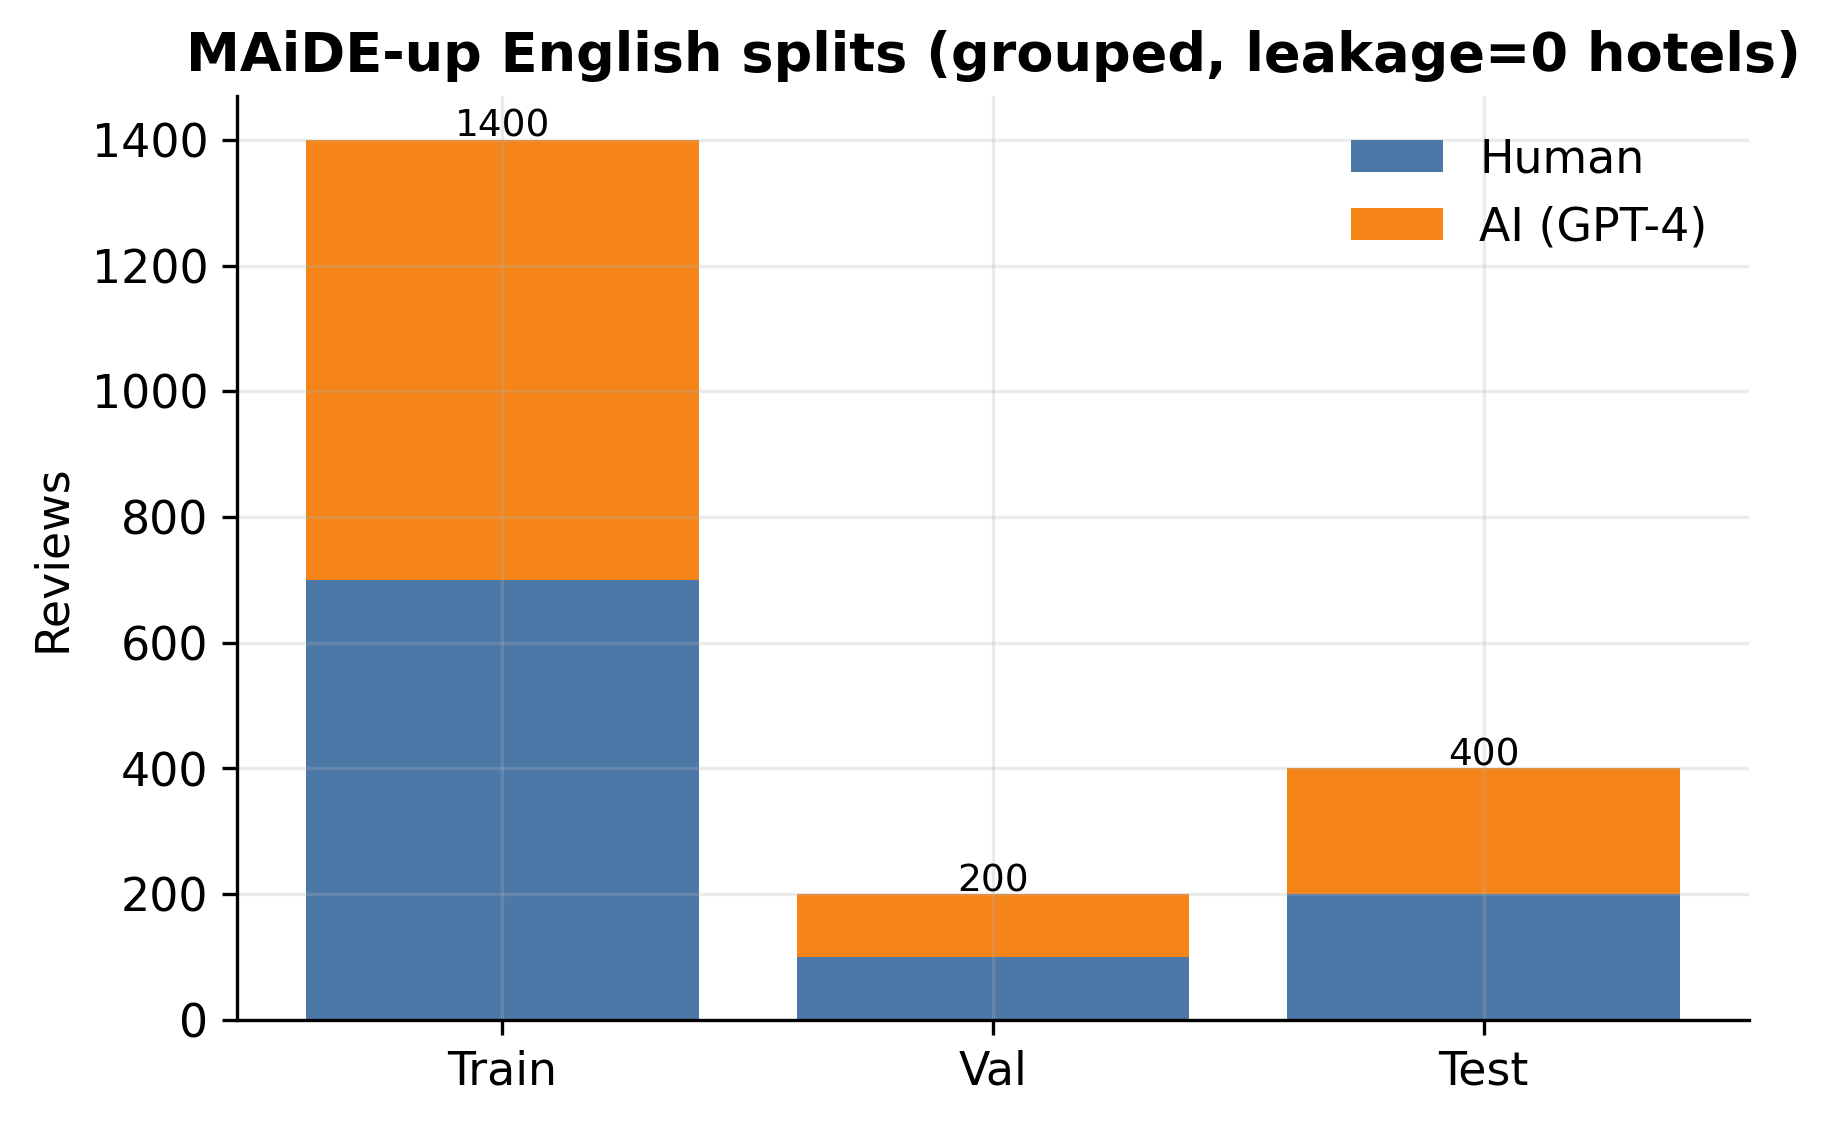
\includegraphics[width=0.6\linewidth]{figures/01_dataset_overview.png}
\caption{MAiDE-up English splits (grouped, zero train--test hotel leakage).}
\label{fig:01_dataset_overview}
\end{figure}
\section{Results}
\subsection{In-domain performance}
\begin{table}[H]\centering
\caption{In-domain performance (mean $\pm$ 95\% CI over seeds; \% units).}
\label{tab:indomain}
\small
\begin{tabular}{lccc}
\toprule
Model & F1 (macro) & ROC-AUC & Accuracy \\
\midrule
Baseline & 93.7 $\pm$ 2.8 & 99.4 $\pm$ 0.3 & 93.8 $\pm$ 2.8 \\
SoftReg & 93.8 $\pm$ 3.6 & 99.3 $\pm$ 0.4 & 93.8 $\pm$ 3.5 \\
Hard-Mask (FAITH) & 93.6 $\pm$ 1.7 & 98.6 $\pm$ 0.6 & 93.6 $\pm$ 1.7 \\
tfidf\_lr & 92.2 & 97.9 & 92.2 \\
tfidf\_lr\_content & 91.7 & 97.2 & 91.8 \\
\bottomrule
\end{tabular}
\end{table}
On in-distribution data the three neural variants are statistically indistinguishable (McNemar baseline vs.\ Hard-Mask, $p=0.15$); Hard-Mask attains the same F1 as the unconstrained baseline, with the tightest interval. Function-word invariance therefore carries no measurable in-domain cost on this benchmark (Figure~\ref{fig:03_indomain_performance}). Confusion matrices (Figure~\ref{fig:04_confusion_matrices}) and ROC/PR curves (Figure~\ref{fig:05_roc_pr}) show the same ordering, with very high ROC-AUC for all neural variants.
\begin{figure}[H]\centering

\includegraphics[width=0.8\linewidth]{figures/03_indomain_performance.png}
\caption{In-domain F1 (mean $\pm$ 95\% CI) with classic baselines.}
\label{fig:03_indomain_performance}
\end{figure}
\begin{figure}[H]\centering

\includegraphics[width=0.95\linewidth]{figures/04_confusion_matrices.png}
\caption{In-domain confusion matrices (reference seed) by variant.}
\label{fig:04_confusion_matrices}
\end{figure}
\begin{figure}[H]\centering

\includegraphics[width=0.95\linewidth]{figures/05_roc_pr.png}
\caption{In-domain ROC and precision--recall curves (reference seed).}
\label{fig:05_roc_pr}
\end{figure}
\subsection{Function-word reliance}
\begin{table}[H]\centering
\caption{Function-word reliance: lower is less reliance.}
\label{tab:reliance}
\small
\begin{tabular}{lcc}
\toprule
Variant & FW attribution mass (IG) & Identity-sensitivity $|\Delta p|$ \\
\midrule
Baseline & 36.5\% & 10.93\% \\
SoftReg & 30.0\% & 10.61\% \\
Hard-Mask (FAITH) & 0.0\% & 0.72\% \\
\bottomrule
\end{tabular}
\end{table}
The unconstrained baseline places a substantial share of its attribution on function words; soft regularisation reduces it; hard masking eliminates it (Figure~\ref{fig:08_fw_attribution_mass}). The forward-only identity-sensitivity metric---the change in AI probability when function words are swapped---agrees: it is near zero for Hard-Mask and clearly positive for the baseline (Figure~\ref{fig:08b_fw_identity_sensitivity}). The two metrics are consistent because they measure the same property (reliance on function-word identity) from gradient and perturbation perspectives.
\begin{figure}[H]\centering
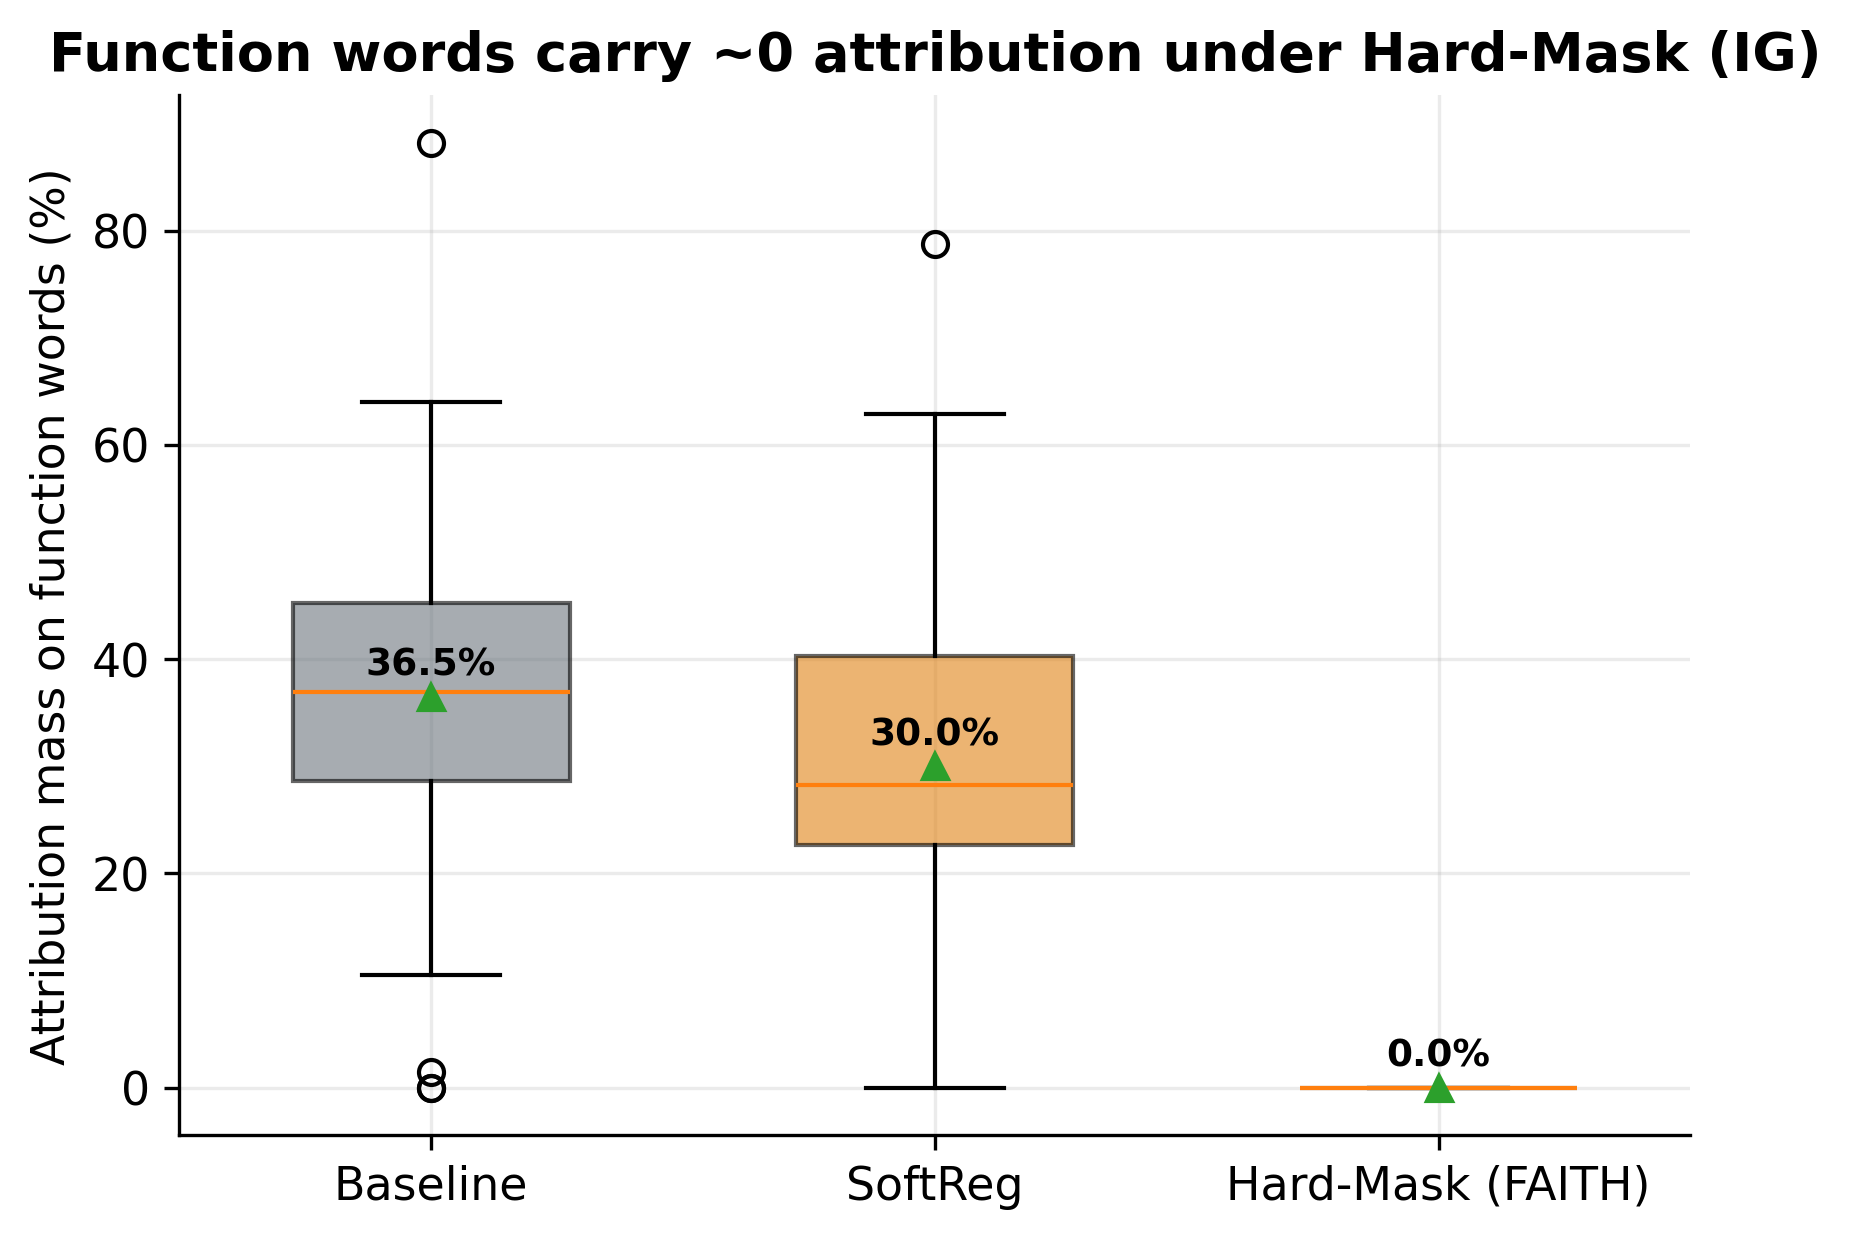
\includegraphics[width=0.72\linewidth]{figures/08_fw_attribution_mass.png}
\caption{Integrated-Gradients attribution mass on function words.}
\label{fig:08_fw_attribution_mass}
\end{figure}
\begin{figure}[H]\centering

\includegraphics[width=0.72\linewidth]{figures/08b_fw_identity_sensitivity.png}
\caption{Change in AI probability when function words are swapped.}
\label{fig:08b_fw_identity_sensitivity}
\end{figure}
\subsection{Robustness to text attacks}
\begin{table}[H]\centering
\caption{F1 (macro) under text attacks (mean over seeds; \% units).}
\label{tab:robust}
\small
\begin{tabular}{lccc}
\toprule
Variant & Clean & function word & synonym \\
\midrule
Baseline & 93.7 & 87.2 & 88.4 \\
SoftReg & 93.8 & 87.0 & 86.4 \\
Hard-Mask (FAITH) & 93.6 & 95.8 & 89.9 \\
\bottomrule
\end{tabular}
\end{table}
Under the function-word attack, the baseline and soft variants lose several points whereas Hard-Mask is essentially unaffected---perturbing function words cannot move a decision that ignores them. Under synonym substitution all variants degrade, but Hard-Mask degrades least and retains the highest F1 (Figure~\ref{fig:07_robustness}). These are the clearest empirical benefits of invariance; we do not claim improvements beyond the two attacks tested.
\begin{figure}[H]\centering

\includegraphics[width=0.8\linewidth]{figures/07_robustness.png}
\caption{F1 under text attacks; Hard-Mask is flat under the function-word attack.}
\label{fig:07_robustness}
\end{figure}
\subsection{Cross-domain and cross-generator transfer}
\begin{table}[H]\centering
\caption{In-domain vs.\ cross-domain OOD (mean $\pm$ 95\% CI; \% units).}
\label{tab:ood}
\small
\begin{tabular}{lcc}
\toprule
Variant & In-domain F1 & OOD F1 (RAID reviews) \\
\midrule
Baseline & 93.7 $\pm$ 2.8 & 69.5 $\pm$ 7.5 \\
SoftReg & 93.8 $\pm$ 3.6 & 68.2 $\pm$ 10.1 \\
Hard-Mask (FAITH) & 93.6 $\pm$ 1.7 & 47.4 $\pm$ 8.3 \\
\bottomrule
\end{tabular}
\end{table}
On the cross-domain OOD set (hotel $\rightarrow$ movie reviews) the picture reverses: Hard-Mask transfers \emph{worse} than the baseline, with non-overlapping confidence intervals (Figure~\ref{fig:06_ood_transfer}). When the content vocabulary shifts, the content words Hard-Mask depends on largely disappear, while the baseline's function-word and stylistic cues evidently carry domain-general signal. Function words are thus not pure noise; in cross-domain transfer they can be useful. The per-generator breakdown (Figure~\ref{fig:06b_cross_generator}) shows the same ordering across most generators. We emphasise a confound: this OOD shifts both domain and generator at once and is an extreme content change, so it does not isolate cross-generator transfer; a same-domain, different-generator test would be needed for that claim.
\begin{figure}[H]\centering

\includegraphics[width=0.8\linewidth]{figures/06_ood_transfer.png}
\caption{In-domain vs.\ cross-domain OOD F1 by variant (mean $\pm$ 95\% CI).}
\label{fig:06_ood_transfer}
\end{figure}
\begin{figure}[H]\centering
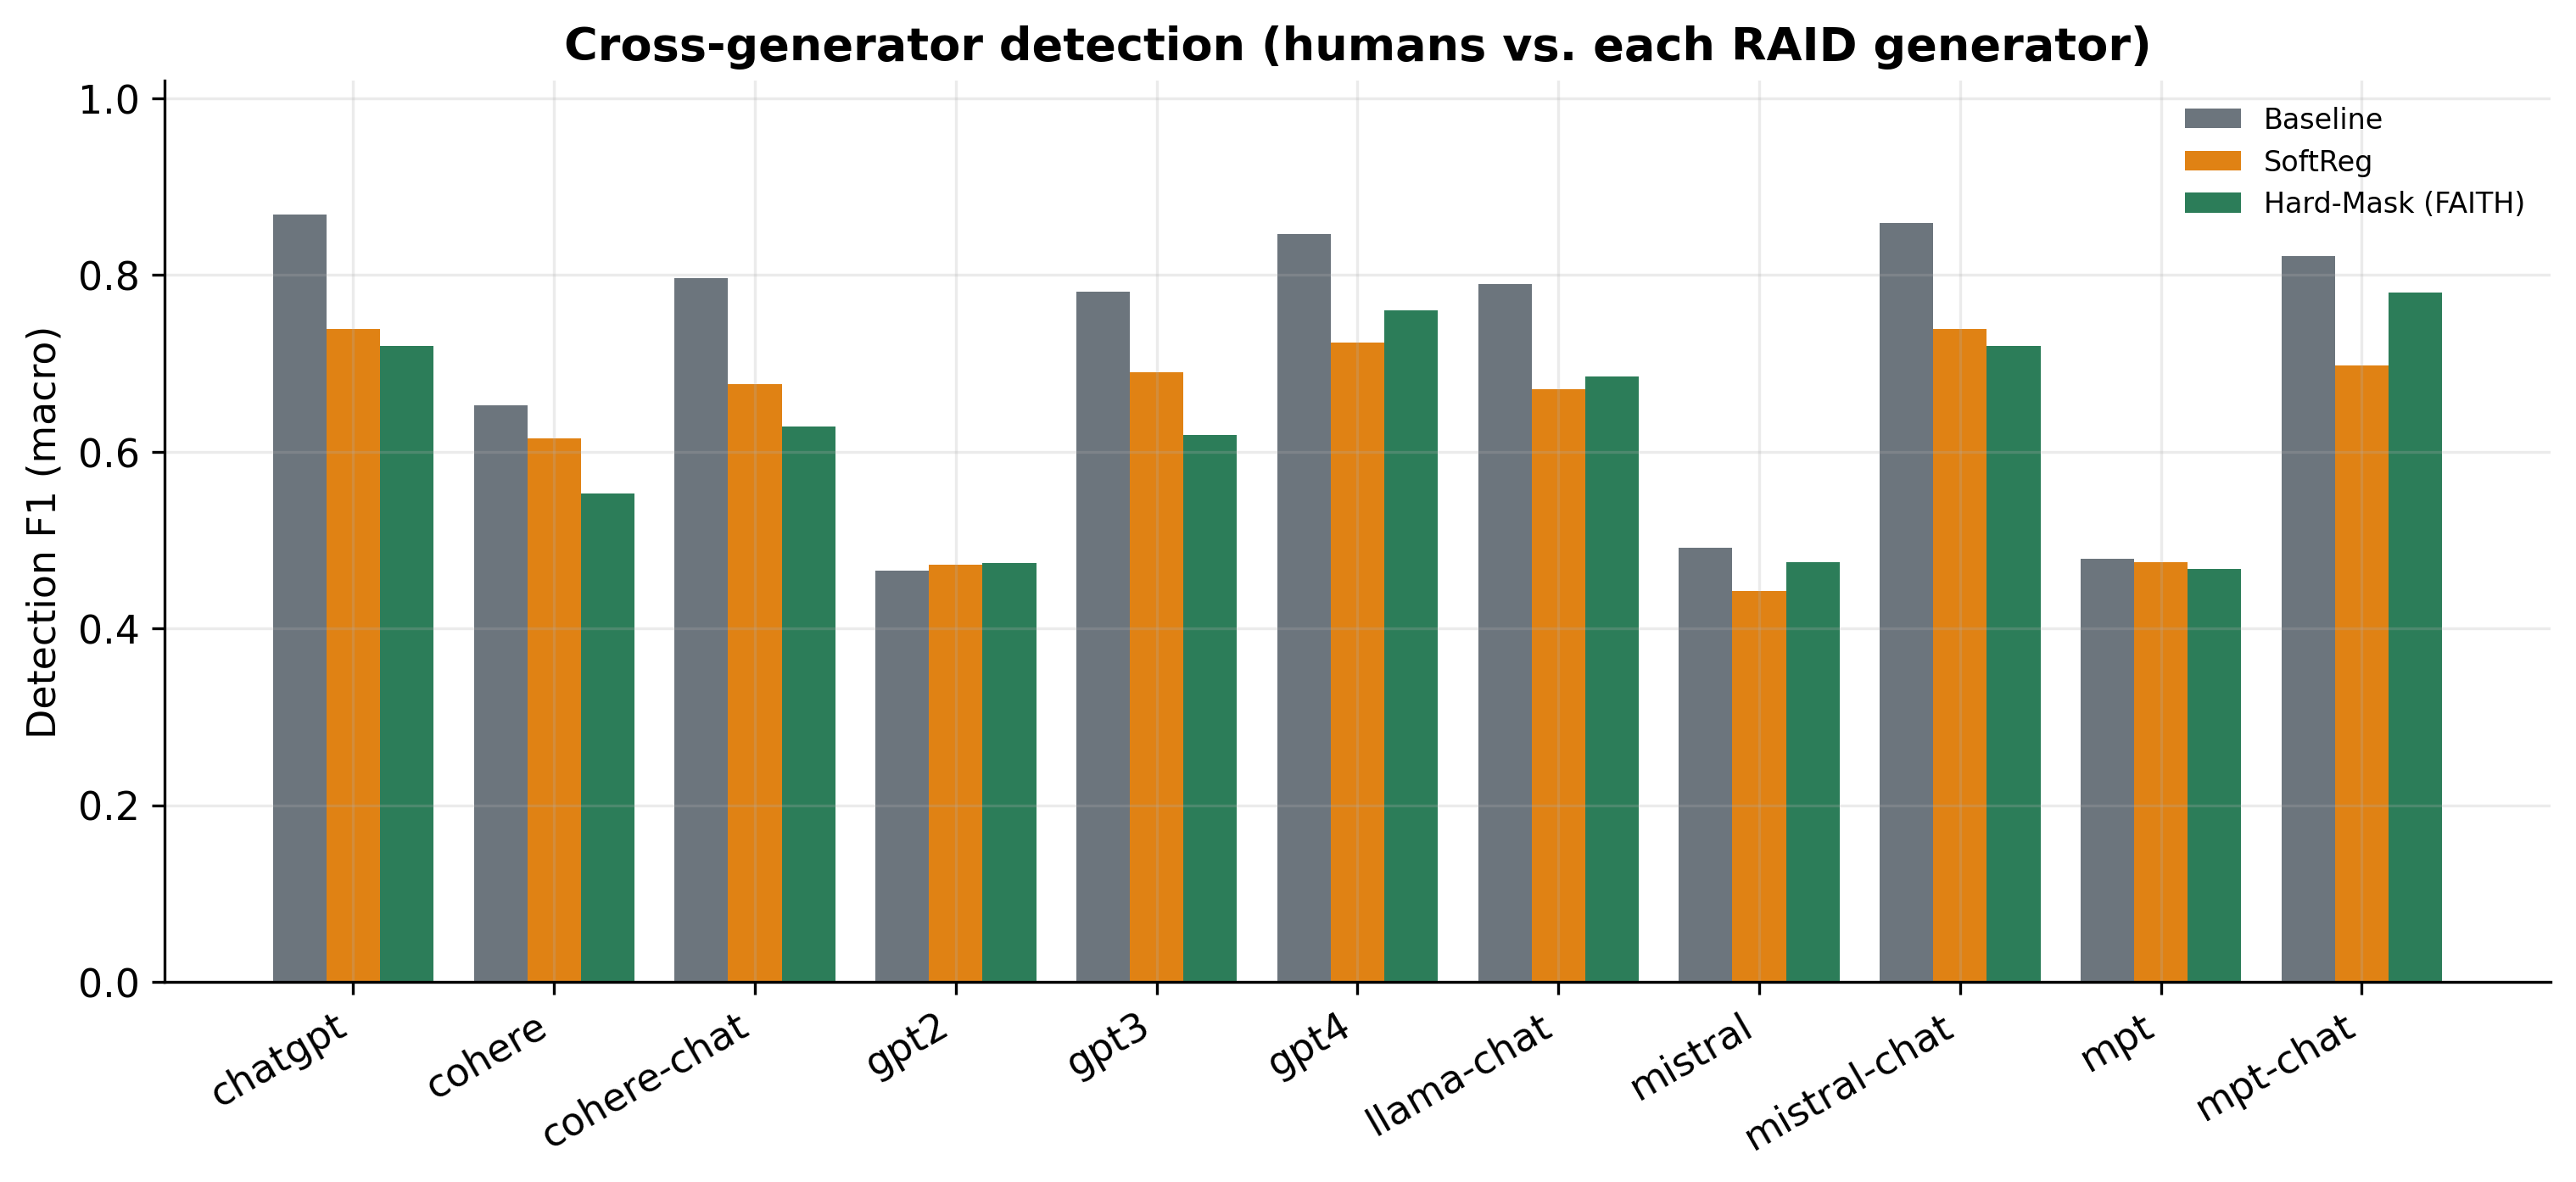
\includegraphics[width=0.95\linewidth]{figures/06b_cross_generator.png}
\caption{Per-generator detection F1 on RAID reviews.}
\label{fig:06b_cross_generator}
\end{figure}
\subsection{Explanation faithfulness}
\begin{table}[H]\centering
\caption{Explanation faithfulness (Integrated Gradients, content words).}
\label{tab:faith}
\small
\begin{tabular}{lcccc}
\toprule
Variant & Compr.\,$\uparrow$ & Suff.\,$\downarrow$ & Del-AUC\,$\downarrow$ & Ins-AUC\,$\uparrow$ \\
\midrule
Baseline & 0.100 & 0.100 & 0.895 & 0.891 \\
SoftReg & 0.047 & 0.054 & 0.900 & 0.904 \\
Hard-Mask (FAITH) & 0.029 & -0.000 & 0.929 & 0.972 \\
\bottomrule
\end{tabular}
\end{table}
Faithfulness is comparable across variants and mixed in direction (Figure~\ref{fig:09_faithfulness}): no variant dominates on all four measures, with Hard-Mask strongest on sufficiency and insertion and the baseline stronger on comprehensiveness. Deletion/insertion curves (Figure~\ref{fig:10_deletion_insertion_curves}) tell the same story. We therefore do \emph{not} claim a faithfulness improvement from invariance; the explanation contribution is structural---explanations are content-only by construction and computed on the deployed model (Figure~\ref{fig:14_example_explanation})---rather than a higher faithfulness score.
\begin{figure}[H]\centering

\includegraphics[width=0.8\linewidth]{figures/09_faithfulness.png}
\caption{ERASER comprehensiveness/sufficiency and deletion/insertion AUC.}
\label{fig:09_faithfulness}
\end{figure}
\begin{figure}[H]\centering
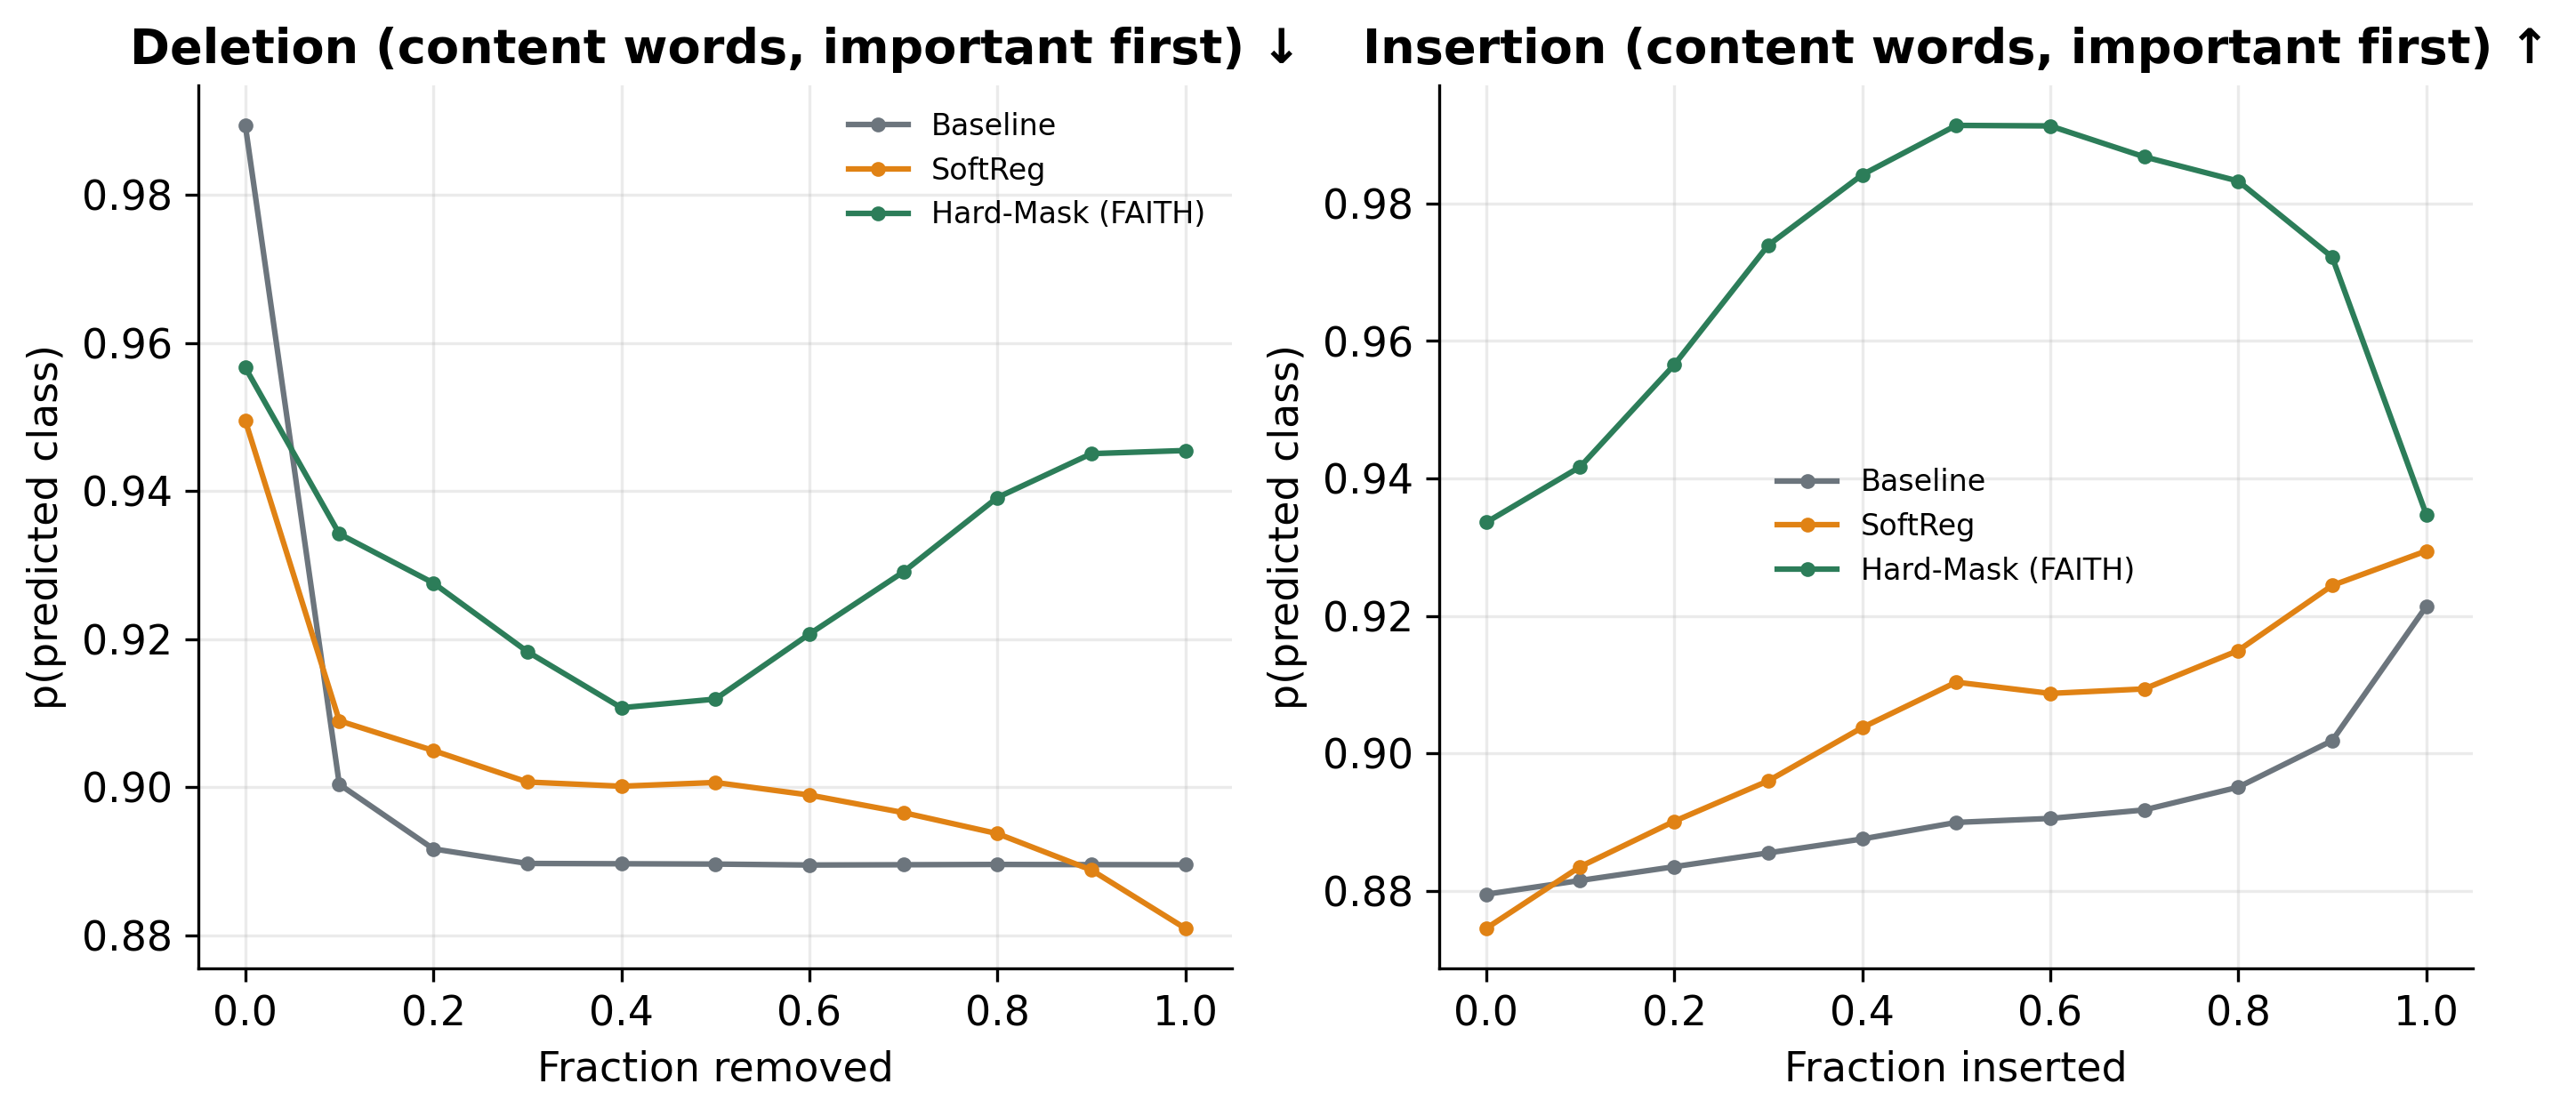
\includegraphics[width=0.95\linewidth]{figures/10_deletion_insertion_curves.png}
\caption{Mean deletion and insertion curves over content words.}
\label{fig:10_deletion_insertion_curves}
\end{figure}
\begin{figure}[H]\centering

\includegraphics[width=0.95\linewidth]{figures/14_example_explanation.png}
\caption{Example explanations: content highlighted, function words greyed.}
\label{fig:14_example_explanation}
\end{figure}
\subsection{Calibration and representation}
Reliability diagrams (Figure~\ref{fig:11_calibration}) summarise calibration on the in-domain test set via the expected calibration error \cite{guo}; we report it for completeness rather than as a contribution. A two-dimensional projection of the encoder representations (Figure~\ref{fig:13_embedding_projection}) shows that human and AI reviews are well separated in-domain for all variants.
\begin{figure}[H]\centering

\includegraphics[width=0.6\linewidth]{figures/11_calibration.png}
\caption{Reliability diagrams (in-domain) with expected calibration error.}
\label{fig:11_calibration}
\end{figure}
\begin{figure}[H]\centering
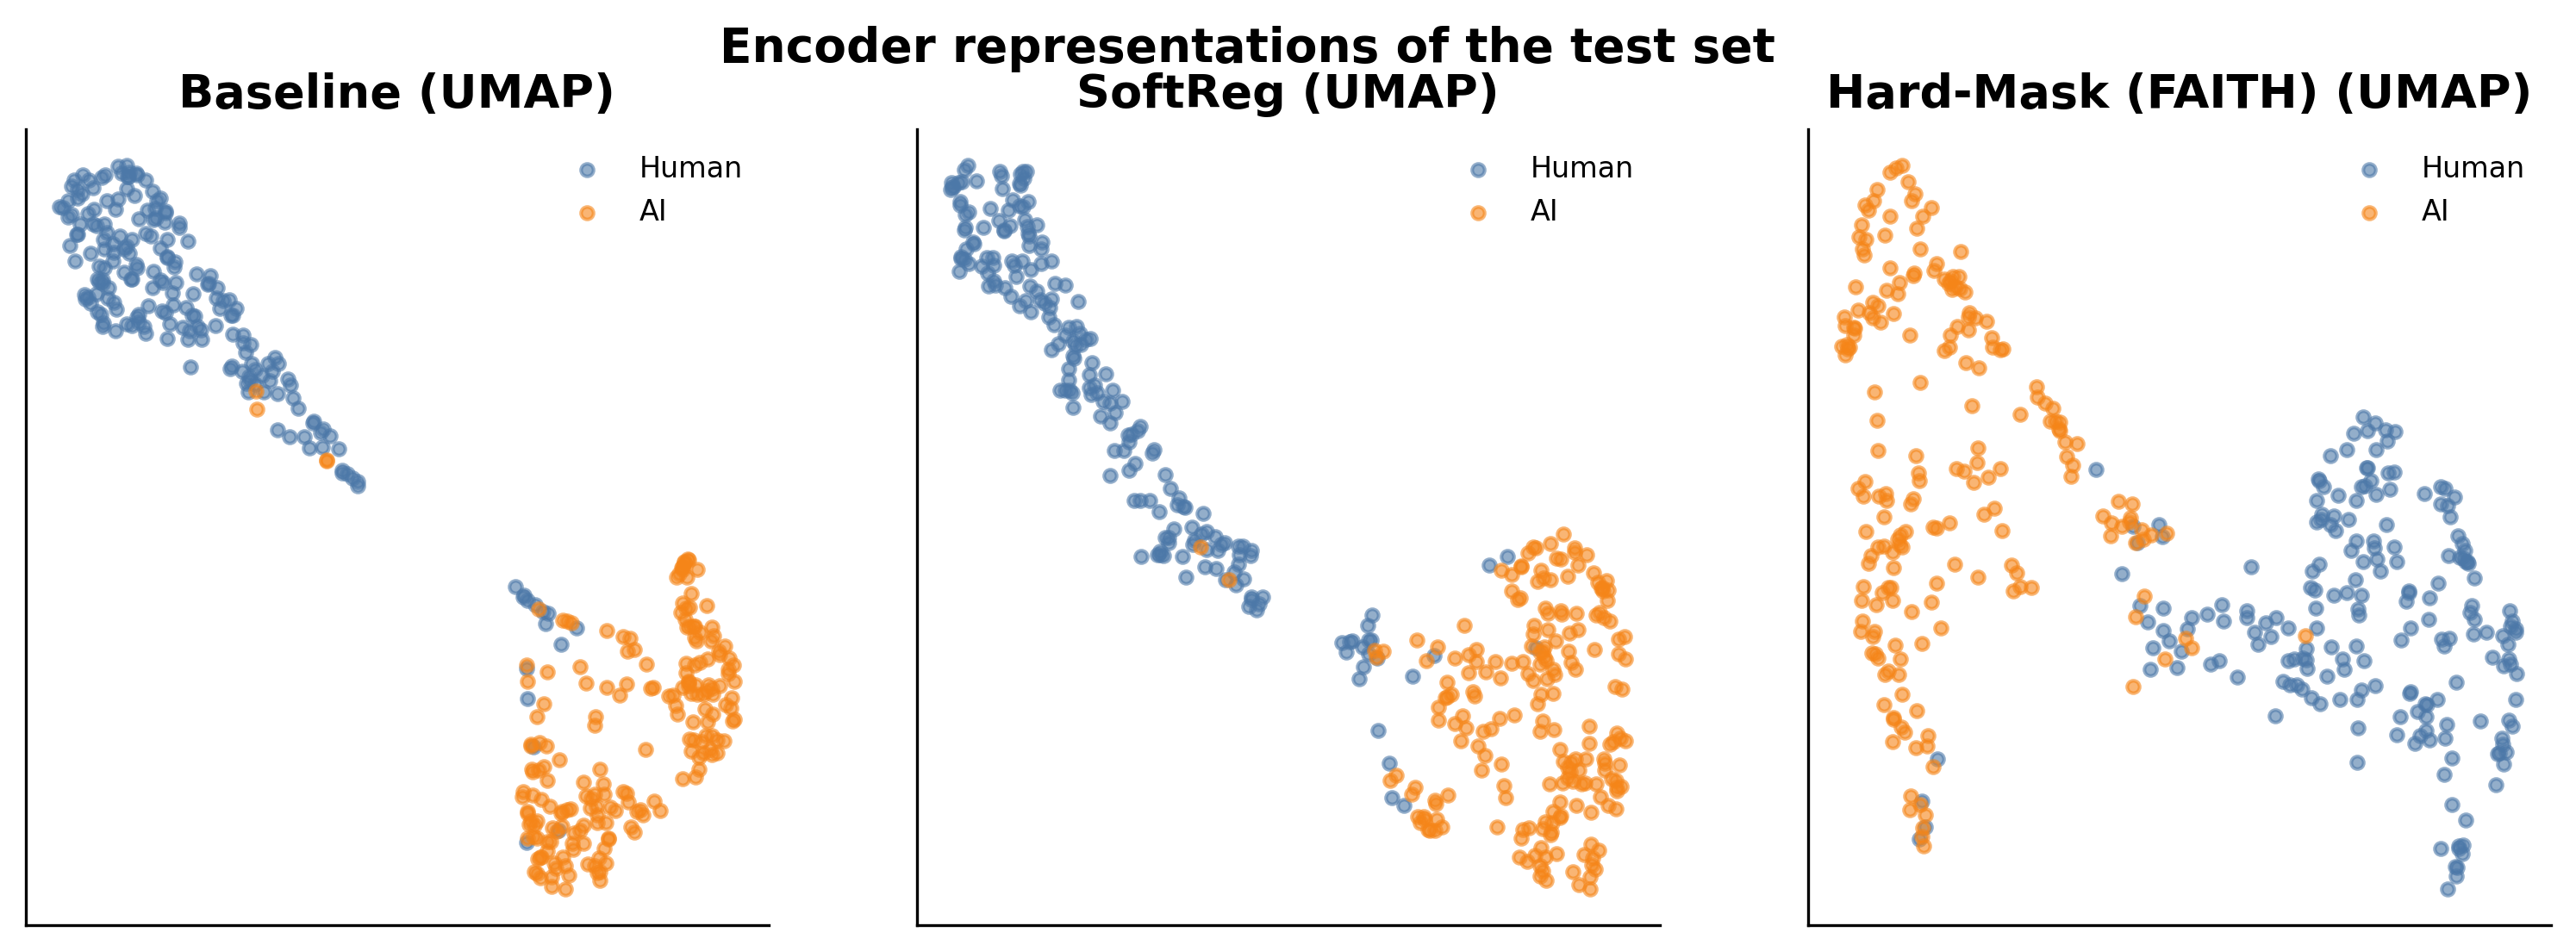
\includegraphics[width=0.95\linewidth]{figures/13_embedding_projection.png}
\caption{2-D projection of encoder representations of the test set.}
\label{fig:13_embedding_projection}
\end{figure}
\subsection{Leakage}
A naive random split inflates baseline F1 to 96.7\% versus 93.2\% under the grouped, leakage-free split (Figure~\ref{fig:02_leakage_gap}). Because hotels recur with both labels, a random split lets the model exploit hotel-specific content; we report grouped numbers throughout and recommend grouped splits for this dataset.
\begin{figure}[H]\centering
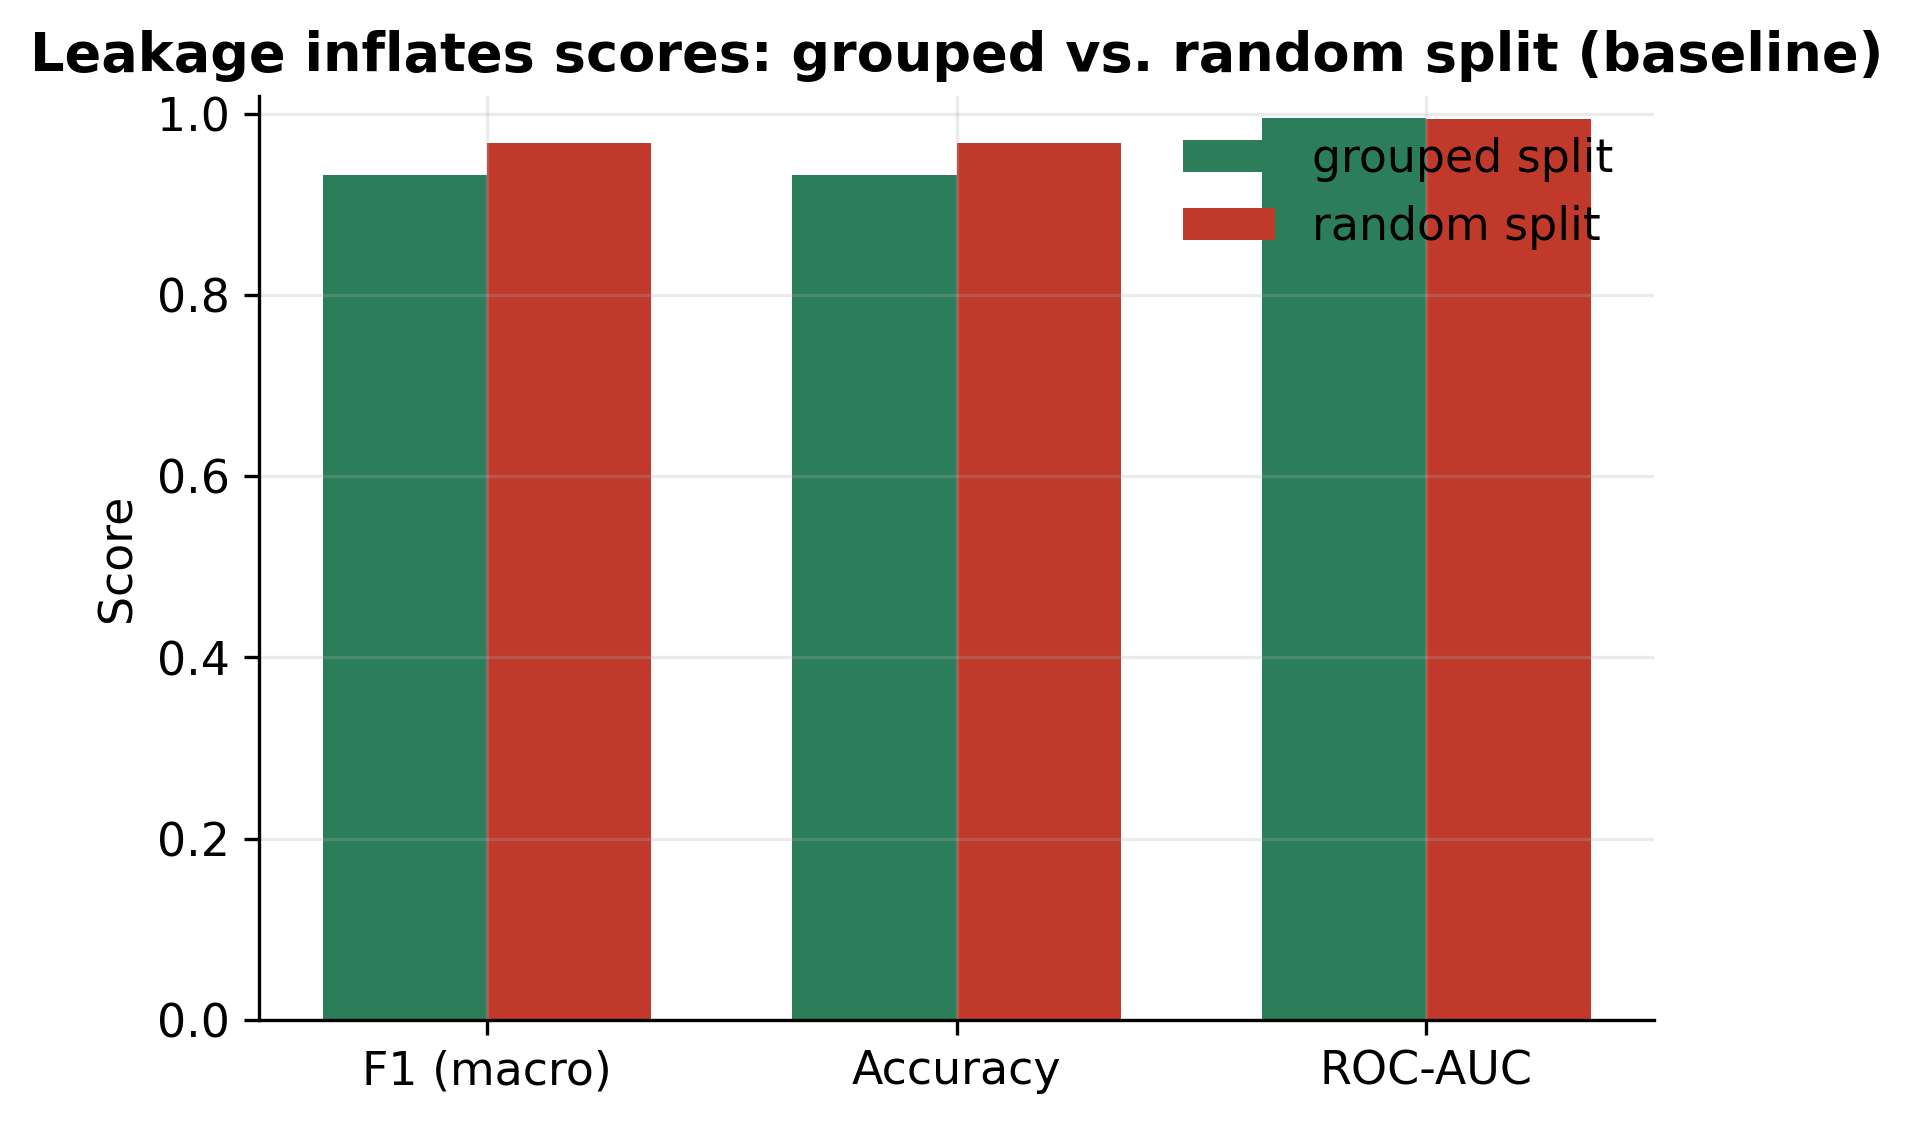
\includegraphics[width=0.6\linewidth]{figures/02_leakage_gap.png}
\caption{Random vs.\ grouped split (baseline): random splitting overstates scores.}
\label{fig:02_leakage_gap}
\end{figure}
\section{Discussion}
Making a detector ignore function words is free in-distribution on this benchmark, yields a provable invariance and the best robustness to the two attacks we test, and produces explanations that are content-only by construction---in contrast to post-hoc, surrogate-based explanations. The cost is cross-domain transfer: when the content vocabulary changes, function-word and stylistic regularities that the constrained model discards carry domain-general signal. Practically, hard masking is attractive where robustness, auditability and a guarantee matter and the domain is fixed; the unconstrained or soft model is preferable for open-domain transfer. We deliberately avoid stronger claims: results are on one in-domain dataset and two attacks, and the OOD evidence is a single benchmark.
\section{Limitations}
The study is English-only and uses a single in-domain generator (GPT-4), so cross-generator evidence comes from a benchmark that also shifts domain and cannot isolate generator effects. The in-domain set is modest (2{,}000 reviews), which widens confidence intervals; we report them honestly rather than selecting favourable seeds. The two attacks are simple proxies for adversarial and paraphrase pressure, not an exhaustive robustness audit. Faithfulness metrics are themselves contested \cite{jacovi} and we do not treat any single one as decisive. Function-word invariance is a design choice with a measured trade-off, not a universally preferable configuration.
\section{Conclusion}
Function words are a measurable shortcut in AI-text detection. A detector that provably ignores them keeps in-domain accuracy, gains robustness to the attacks we test, and explains itself with content alone---at a measured cost to cross-domain transfer. We release code, leakage-free protocols, multi-seed results with confidence intervals, and figures that regenerate from a single results file.
\paragraph{Reproducibility.} All numbers come from a single results JSON; figures and this paper regenerate from it; the hard-masking guarantee is asserted by an automated test. Code: \url{https://github.com/scar09-22/FAITH-Detect}.
\appendix
\section{Training behaviour}
Figure~\ref{fig:12_learning_curves} shows training loss and validation F1 by epoch, averaged over seeds. The soft and hard variants start slower (they discard or down-weight function-word information) but reach comparable validation F1.
\begin{figure}[H]\centering

\includegraphics[width=0.95\linewidth]{figures/12_learning_curves.png}
\caption{Training loss and validation F1 by epoch (mean over seeds).}
\label{fig:12_learning_curves}
\end{figure}
\begin{thebibliography}{99}\small
\bibitem{maideup} O. Ignat, X. Xu, R. Mihalcea. MAiDE-up: Multilingual Deception Detection of AI-Generated Hotel Reviews. Findings of NAACL, 2025.
\bibitem{raid} L. Dugan, A. Hwang, F. Trhlik, et al. RAID: A Shared Benchmark for Robust Evaluation of Machine-Generated Text Detectors. ACL, 2024.
\bibitem{ig} M. Sundararajan, A. Taly, Q. Yan. Axiomatic Attribution for Deep Networks. ICML, 2017.
\bibitem{eraser} J. DeYoung, S. Jain, N. F. Rajani, et al. ERASER: A Benchmark to Evaluate Rationalized NLP Models. ACL, 2020.
\bibitem{ross} A. S. Ross, M. C. Hughes, F. Doshi-Velez. Right for the Right Reasons: Training Differentiable Models by Constraining their Explanations. IJCAI, 2017.
\bibitem{detectgpt} E. Mitchell, Y. Lee, A. Khazatsky, C. D. Manning, C. Finn. DetectGPT: Zero-Shot Machine-Generated Text Detection using Probability Curvature. ICML, 2023.
\bibitem{gltr} S. Gehrmann, H. Strobelt, A. M. Rush. GLTR: Statistical Detection and Visualization of Generated Text. ACL (System Demonstrations), 2019.
\bibitem{rise} V. Petsiuk, A. Das, K. Saenko. RISE: Randomized Input Sampling for Explanation of Black-box Models. BMVC, 2018.
\bibitem{geirhos} R. Geirhos, J.-H. Jacobsen, C. Michaelis, et al. Shortcut Learning in Deep Neural Networks. Nature Machine Intelligence, 2020.
\bibitem{roberta} Y. Liu, M. Ott, N. Goyal, et al. RoBERTa: A Robustly Optimized BERT Pretraining Approach. arXiv:1907.11692, 2019.
\bibitem{lime} M. T. Ribeiro, S. Singh, C. Guestrin. ``Why Should I Trust You?'': Explaining the Predictions of Any Classifier. KDD, 2016.
\bibitem{shap} S. M. Lundberg, S.-I. Lee. A Unified Approach to Interpreting Model Predictions. NeurIPS, 2017.
\bibitem{jacovi} A. Jacovi, Y. Goldberg. Towards Faithfully Interpretable NLP Systems: How Should We Define and Evaluate Faithfulness? ACL, 2020.
\bibitem{sadasivan} V. S. Sadasivan, A. Kumar, S. Balasubramanian, W. Wang, S. Feizi. Can AI-Generated Text be Reliably Detected? arXiv:2303.11156, 2023.
\bibitem{krishna} K. Krishna, Y. Song, M. Karpinska, J. Wieting, M. Iyyer. Paraphrasing Evades Detectors of AI-Generated Text, but Retrieval is an Effective Defense. NeurIPS, 2023.
\bibitem{solaiman} I. Solaiman, M. Brundage, J. Clark, et al. Release Strategies and the Social Impacts of Language Models. arXiv:1908.09203, 2019.
\bibitem{crothers} E. Crothers, N. Japkowicz, H. L. Viktor. Machine-Generated Text: A Comprehensive Survey of Threat Models and Detection Methods. IEEE Access, 2023.
\bibitem{guo} C. Guo, G. Pleiss, Y. Sun, K. Q. Weinberger. On Calibration of Modern Neural Networks. ICML, 2017.
\bibitem{gururangan} S. Gururangan, S. Swayamdipta, O. Levy, et al. Annotation Artifacts in Natural Language Inference Data. NAACL, 2018.
\bibitem{mccoy} T. McCoy, E. Pavlick, T. Linzen. Right for the Wrong Reasons: Diagnosing Syntactic Heuristics in Natural Language Inference. ACL, 2019.
\bibitem{wordnet} G. A. Miller. WordNet: A Lexical Database for English. Communications of the ACM, 1995.
\bibitem{adamw} I. Loshchilov, F. Hutter. Decoupled Weight Decay Regularization. ICLR, 2019.
\bibitem{spacy} M. Honnibal, I. Montani. spaCy: Industrial-Strength Natural Language Processing, 2017.
\end{thebibliography}
\end{document}
